\documentclass[a4paper]{article}

\usepackage{graphicx}
\usepackage{amsmath,amssymb}
\usepackage{minted}
\usepackage{multirow}
\usepackage{float}
\usepackage{todonotes}
\usepackage{forest}
\usepackage{xstring}
\usepackage{xcolor}
\usepackage[most]{tcolorbox}
\usepackage{xparse}
\usepackage{natbib}

\usetikzlibrary{graphs,graphdrawing}
\usegdlibrary{layered}

% for external graphviz
\input{/home/donkarlo/Dropbox/repo/nd_ai_project/src/nd_ai/knoweldge_representation/language/formal/computer/programming/tex/latex/code_clips/external_graphviz.tex}

% for tags
\input{/home/donkarlo/Dropbox/repo/nd_ai_project/src/nd_ai/knoweldge_representation/language/formal/computer/programming/tex/latex/parts/control_sequence/kind/semtag/semtag.tex}

% for links
\input{/home/donkarlo/Dropbox/repo/nd_ai_project/src/nd_ai/knoweldge_representation/language/formal/computer/programming/tex/latex/code_clips/seehere.tex}

\title{}
\date{}

\begin{document}
    \maketitle
    
    \url{https://en.wikipedia.org/wiki/Action_potential}
    Also called as spike
    
    \cite{hodgkin-1952-a-quantitative-description-of-membrane-current-and-its-application-to-conduction-and-excitation-in-nerve} present a quantitative model of nerve membrane current based on sodium, potassium, leakage current, and membrane capacitance.
    The paper formulates voltage-dependent conductance equations that explain action potential generation, propagation, excitation, and refractory behavior.
    Its main contribution is the mathematical foundation of the Hodgkin-Huxley model, connecting ionic membrane dynamics to nerve conduction.
    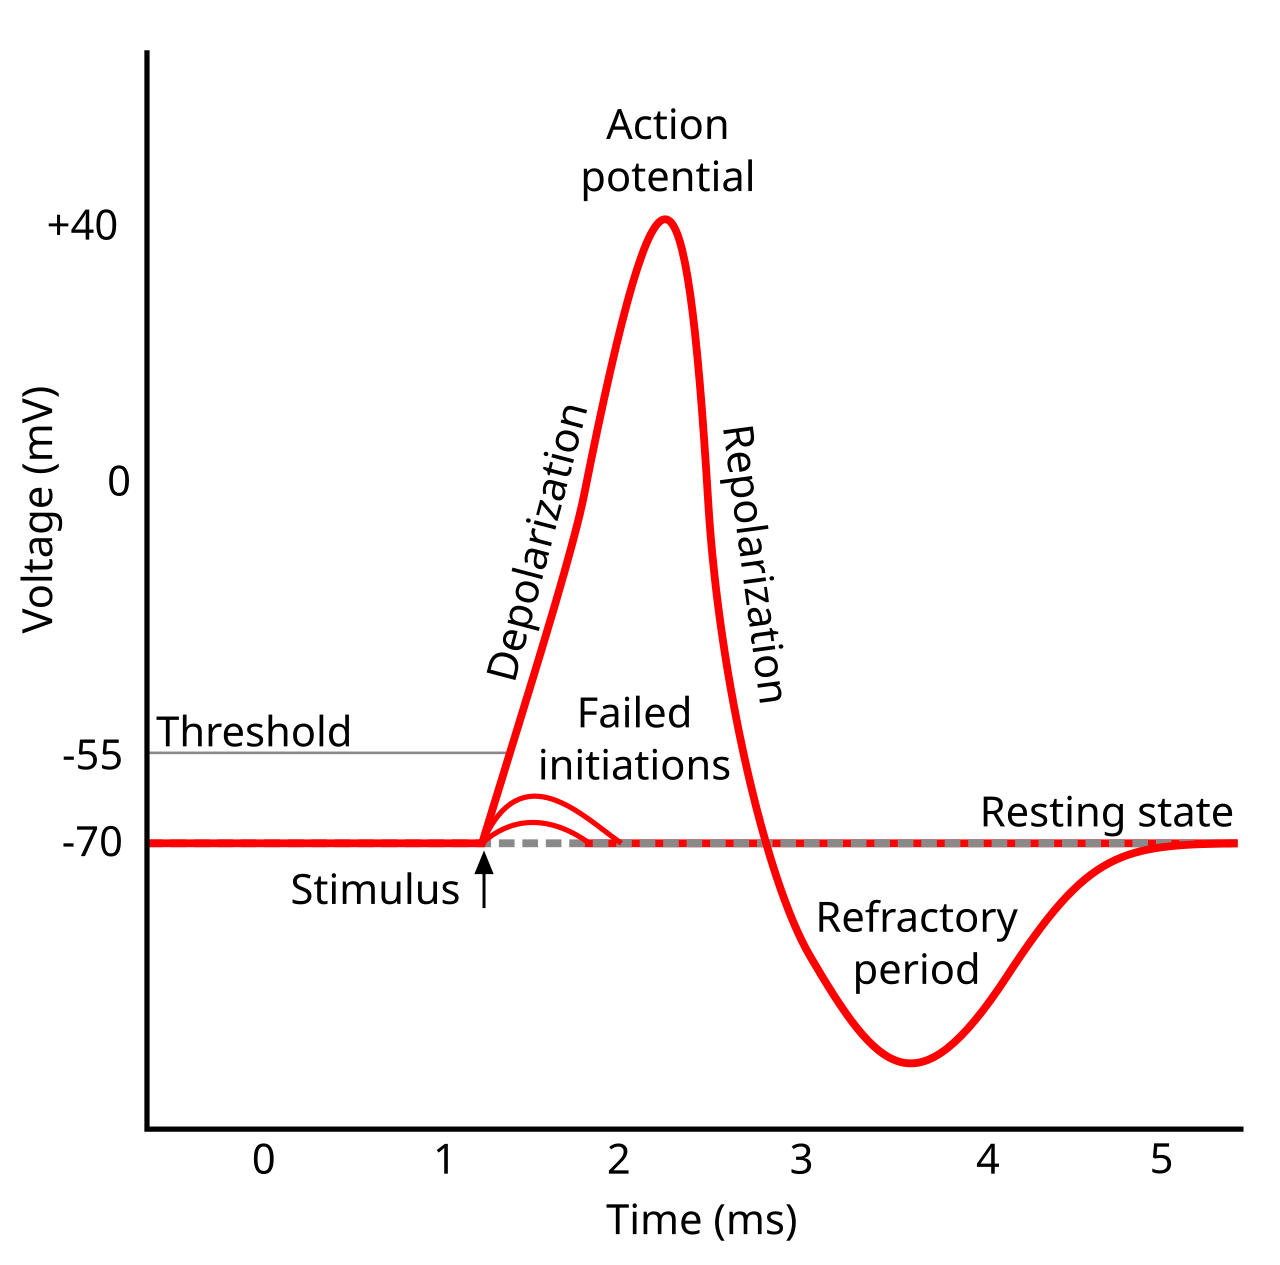
\includegraphics[width=\paperwidth]{action_potential.png}
    %\bibliographystyle{plainnat}
    %\bibliography{/home/donkarlo/Dropbox/repo/nd_shared_research/bibliography/bibliography.bib}
\end{document}
